\documentclass{beamer}

\usetheme{Boadilla}

\usepackage{xifthen}
\usepackage{tikz}
\usetikzlibrary{calc}
\usepackage{amssymb}
\usepackage{algpseudocodex}

\title{Graphes et Algorithmes}
\author{loig.jezequel@univ-nantes.fr}
\date{}

\setbeamertemplate{subsection in toc}[subsections numbered]

\AtBeginSection[]{
    \begin{frame}
        \vfill
        \centering
        \begin{beamercolorbox}[sep=8pt,center,shadow=true,rounded=true]{title}
            \usebeamerfont{title}Partie \thesection~: \insertsectionhead\par%
        \end{beamercolorbox}
        \begin{center}
            \begin{minipage}{5.5cm}
                \tableofcontents[sections=\value{section}, sectionstyle=hide]
            \end{minipage}
        \end{center}
        \vfill
    \end{frame}
}

\AtBeginSubsection[]{
    \begin{frame}
        \vfill
        \centering
        \begin{beamercolorbox}[sep=8pt,center,shadow=true,rounded=true]{title}
            \usebeamerfont{title}\thesection.\thesubsection~\insertsubsectionhead\par%
        \end{beamercolorbox}
        \vfill
    \end{frame}
}

\newcommand{\enavant}[1]{\textcolor{red}{#1}}

% defs, exercices, etc
\newcommand{\notation}[2][]{
    \begin{block}{Notation\ifthenelse{\NOT\isempty{#1}}{~: #1}{}}
        #2
    \end{block}
}

\renewcommand{\definition}[2][]{
    \begin{block}{Définition\ifthenelse{\NOT\isempty{#1}}{~: #1}{}}
        #2
    \end{block}
}

\newcommand{\exercice}[2][]{
    \begin{exampleblock}{Exercice\ifthenelse{\NOT\isempty{#1}}{~: #1}{}}
        #2
    \end{exampleblock}
}

\newcommand{\proposition}[2][]{
    \begin{alertblock}{Proposition\ifthenelse{\NOT\isempty{#1}}{~: #1}{}}
        #2
    \end{alertblock}
}

\newcommand{\remarque}[2][]{
    \begin{alertblock}{Remarque\ifthenelse{\NOT\isempty{#1}}{~: #1}{}}
        #2
    \end{alertblock}
}

% notations
\newcommand{\arcs}{E}
\newcommand{\arc}{e}
\newcommand{\arcvers}[1]{t(#1)}
\newcommand{\arcdepuis}[1]{f(#1)}
\newcommand{\sommets}{V}
\newcommand{\sommet}{v}
\newcommand{\sommetb}{v'}
\newcommand{\sommetc}{v"}
\newcommand{\pre}[1]{#1^-}
\newcommand{\suc}[1]{#1^+}
\newcommand{\graphe}{G}
\newcommand{\graphefunc}{\mathcal{G}}
\newcommand{\graphedef}{\graphe{} = (\sommets{}, \arcs{})}
\newcommand{\taille}[1]{|#1|}
\newcommand{\adjmat}[1]{\mathcal{A}_{#1}}
\newcommand{\adjmatelem}{a_{ij}}
\newcommand{\incmat}[1]{\mathcal{I}_{#1}}
\newcommand{\incmatelem}{\textrm{\sc i}_{ij}}
\newcommand{\voisins}[1]{N(#1)}
\newcommand{\degnot}{d}
\newcommand{\degre}[1]{\degnot{}(#1)}
\newcommand{\dege}[1]{\degnot{}^-(#1)}
\newcommand{\degs}[1]{\degnot{}^+(#1)}
\newcommand{\relation}{R}
\newcommand{\ensemble}{X}
\newcommand{\cheminvers}{\rightsquigarrow}
\newcommand{\chemin}{w}
\newcommand{\graphechem}{\graphe{}^+}
\newcommand{\arcschem}{\arcs{}^+}
\newcommand{\sommetschem}{\sommets{}^+}
\newcommand{\graphechemdef}{\graphechem{}=(\sommetschem{}, \arcschem{})}
\newcommand{\infgraphe}{\leq_G}
\newcommand{\sufgraphe}{\geq_G}
\newcommand{\uniong}{\cup_G}
\newcommand{\compog}{\circ_G}
\newcommand{\suiteelem}[1]{P_{#1}}
\newcommand{\suitepuiss}{(\suiteelem{n})}
\newcommand{\hornerelem}[1]{R_{#1}}
\newcommand{\horner}{(\hornerelem{n})}
\newcommand{\roy}[1]{\vartheta_{#1}}
\newcommand{\route}{\rho}
\newcommand{\distance}[2]{d(#1,#2)}
\newcommand{\cout}{c}
\newcommand{\grapheval}{\graphe{} = (\sommets{}, \arcs{}, \cout{})}
\newcommand{\pbvv}{$\sommet{}-opt-\sommetb{}$}
\newcommand{\pbvetoile}{$\sommet{}-opt-*$}
\newcommand{\pbetoileetoile}{$*-opt-*$}

% algos
\newcommand{\In}[1]{\State {\bf input} #1}
\newcommand{\Out}[1]{\State {\bf output} #1}

% dessins
\newcommand{\shiftdraw}[4]{\draw[shorten >=7pt, shorten <=7pt, -latex] let \p1 = (#1), \p2 = (#2) in [shift={(#3, #4)}] (\p1) -- (\p2)}

\begin{document}

    \frame{
        \maketitle{}
    }

    \section{Présentation du cours}

\frame{
    \frametitle{Organisation du cours}

    \begin{block}{Organisation des séances}
        \begin{description}
            \item[CM~:] notions de base sur les graphes, présentation d'algorithmes classiques, exemple de présentation
            \item[TD~:] travail de recherche par groupe sur une application des graphes ou un sujet théorique plus avancé, présentation au reste de la classe
        \end{description}
    \end{block}

    \begin{block}{Évaluation}
        \begin{description}
            \item[50\%] tests sur le cours en début de séances
            \item[50\%] présentation des sujets de TD
        \end{description}
    \end{block}
}

\frame{
    \frametitle{Pourquoi étudier les graphes}

    \begin{block}{Graphe}
        Outil de \enavant{modélisation} permettant de représenter les relations entre les éléments d'un ensemble fini :
        \begin{itemize}
            \item routes et distances entre villes,
            \item liens hypertext entre pages web,
            \item etc
        \end{itemize}
    \end{block}

    \begin{block}{Algoritmes}
        Pour analyser les relations représentées par un graphe :
        \begin{itemize}
            \item trouver le plus court trajet entre deux villes,
            \item étudier les groupes sociaux sur internet,
            \item etc
        \end{itemize}
    \end{block}
}

\frame{
    \frametitle{Exemple d'application~: théorème des 4 couleurs}
    \hspace*{-0.5cm}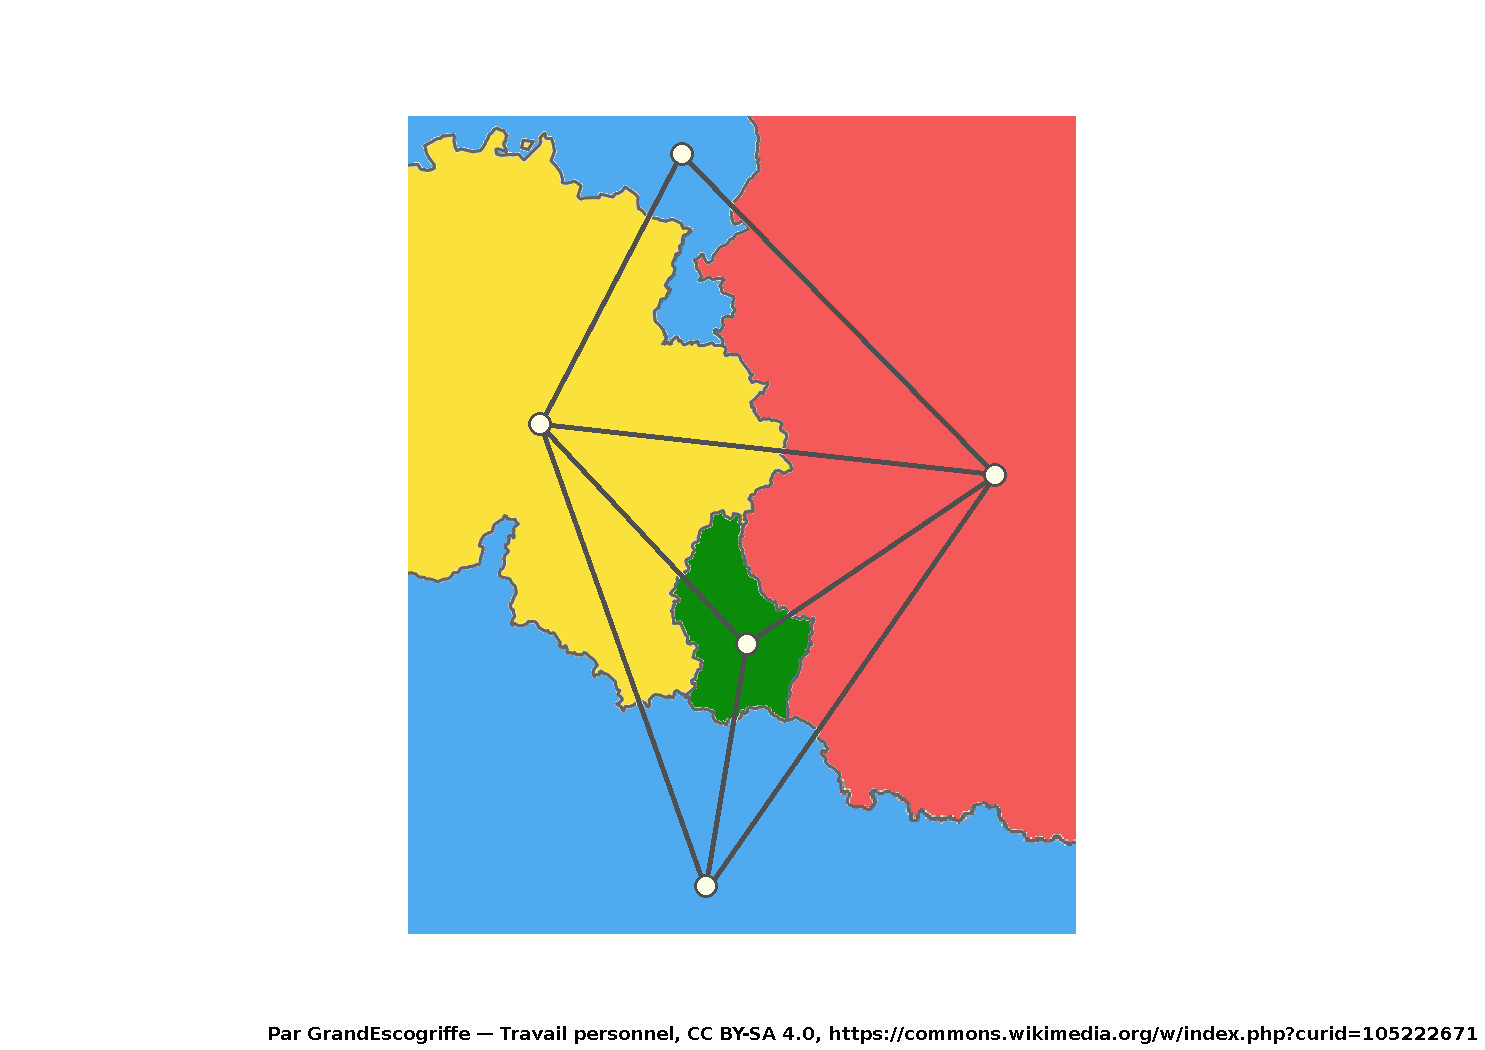
\includegraphics[width=12cm]{1-quatrecouleurs.jpg}
}

\frame{
    \frametitle{Exemple d'application~: sortir d'un labyrinthe}
    \hspace*{-0.5cm}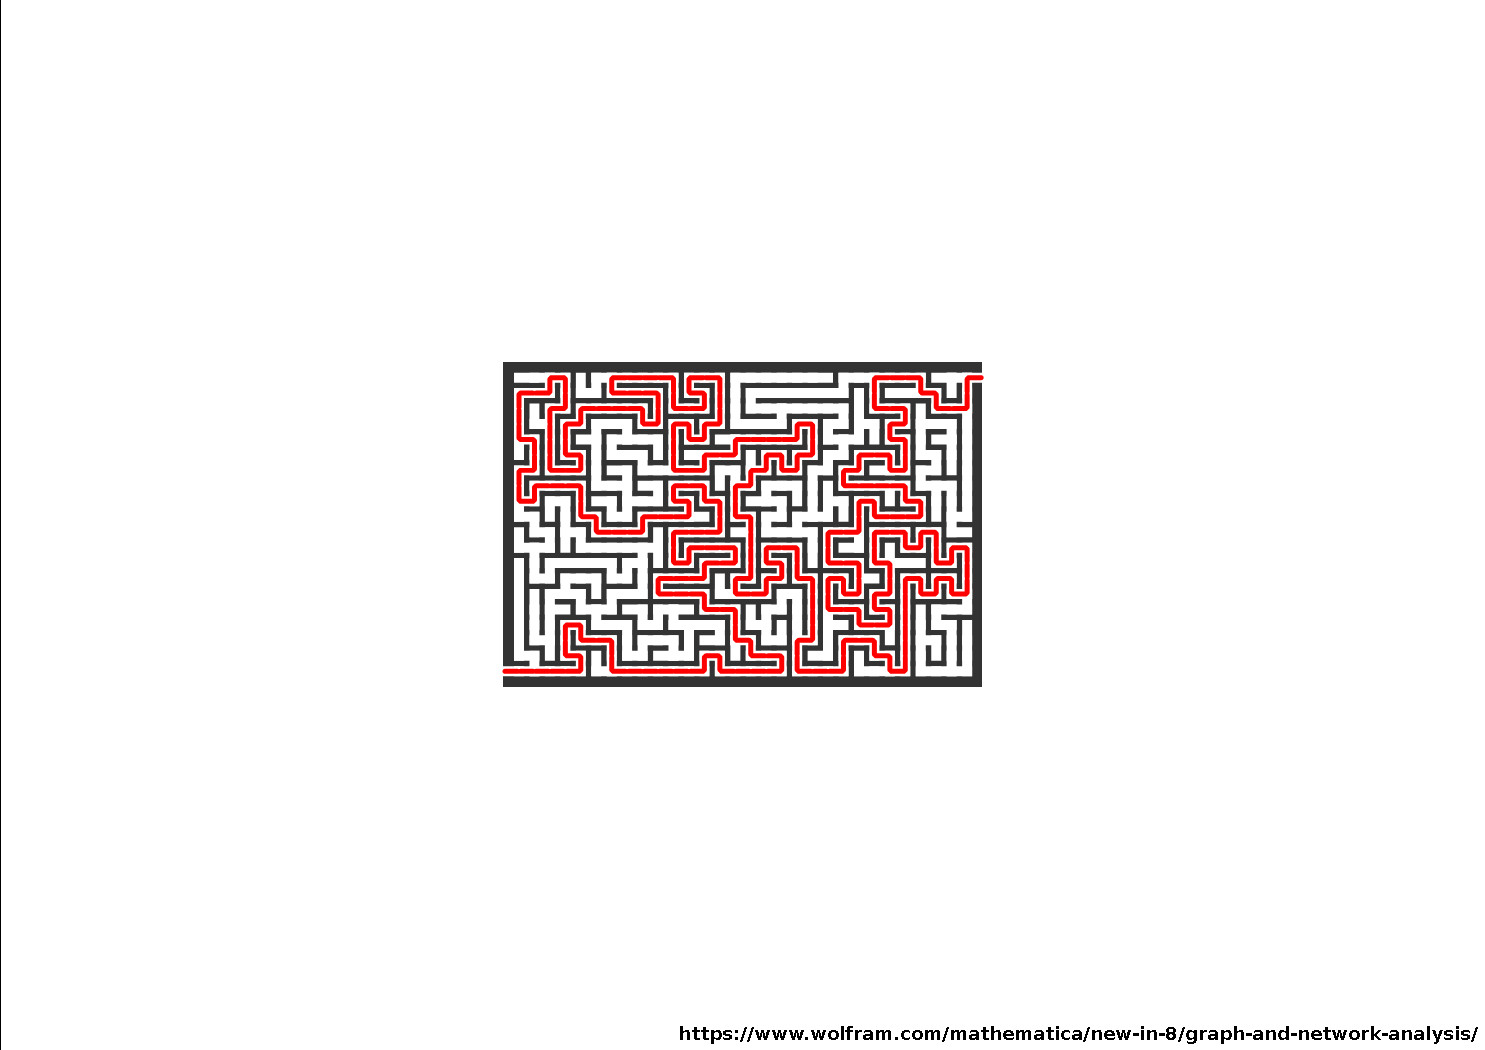
\includegraphics[width=12cm]{2-lab.jpg}
}

\frame{
    \frametitle{Exemple d'application~: recherche d'itinéraire}
    \hspace*{-0.5cm}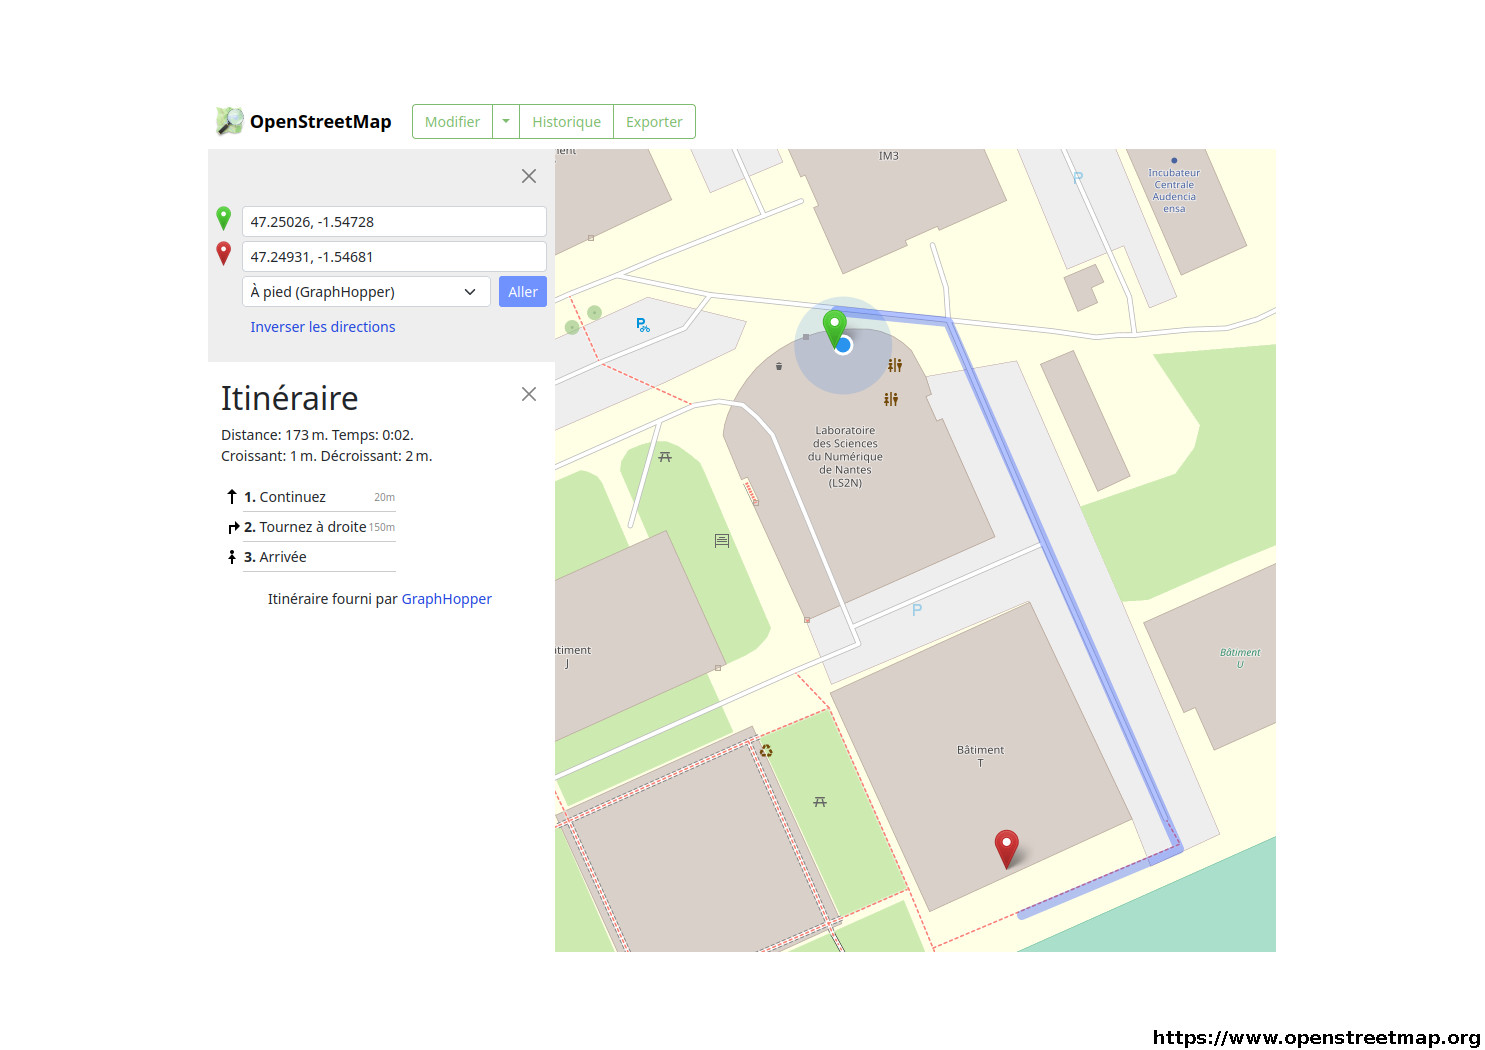
\includegraphics[width=12cm]{3-map.jpg}
}

\frame{
    \frametitle{Exemple d'application~: représentation du web}
    \hspace*{-0.5cm}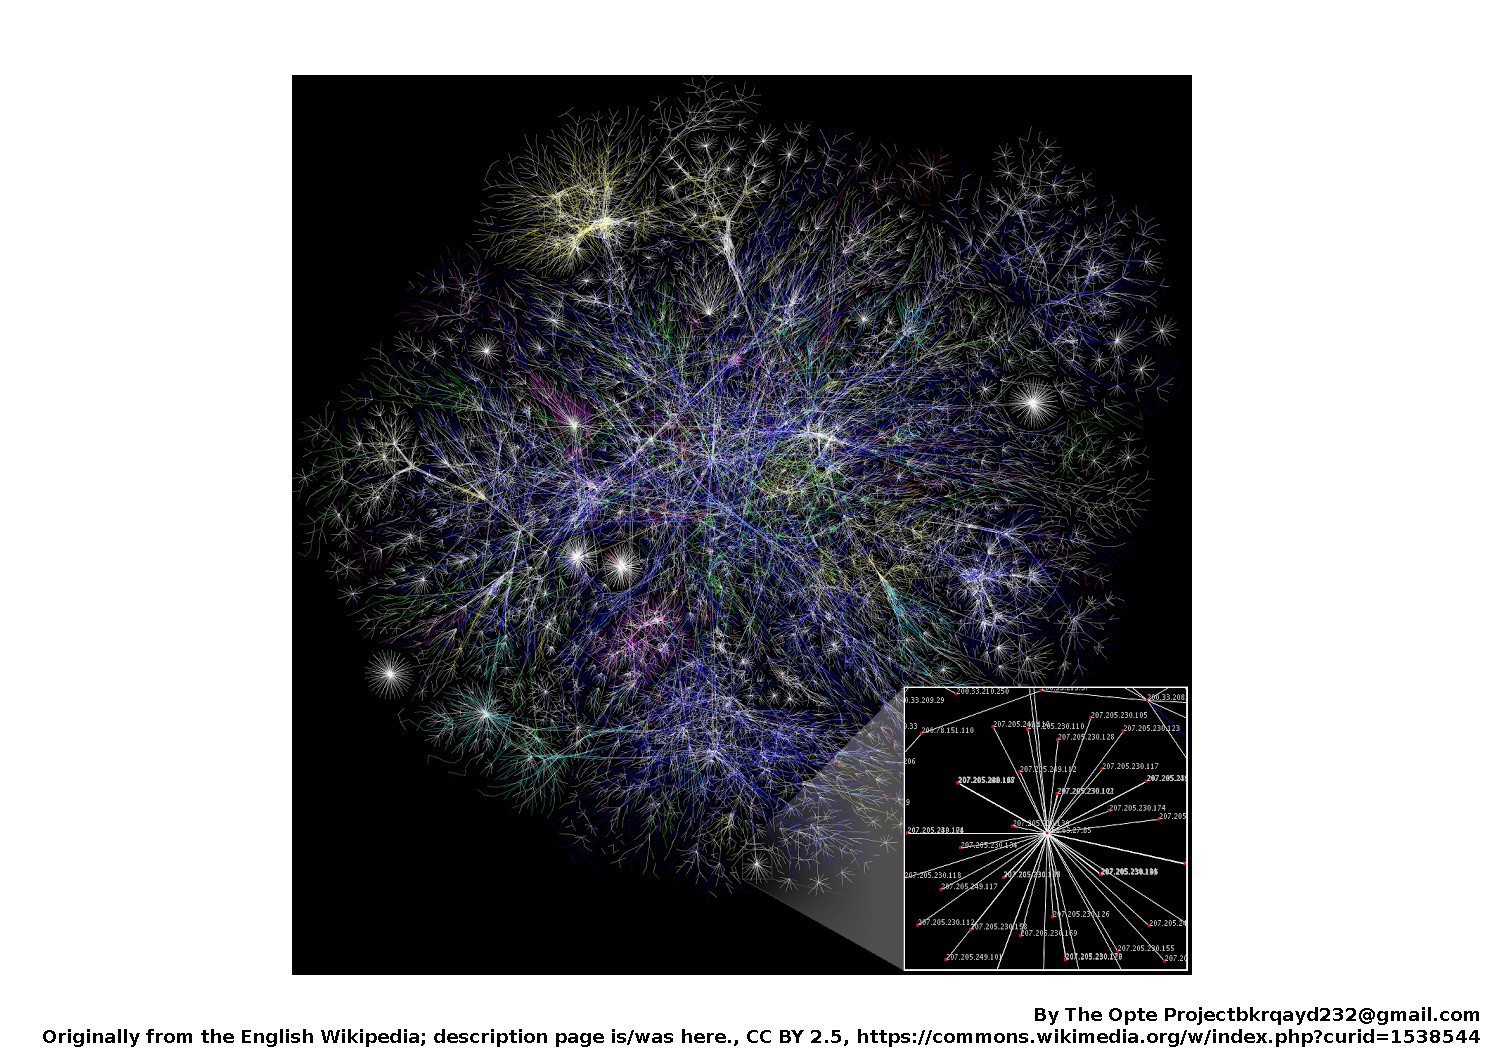
\includegraphics[width=12cm]{4-carteduweb.jpg}
}

\frame{
    \frametitle{Exemple d'application~: réseaux neuronaux}
    \hspace*{-0.5cm}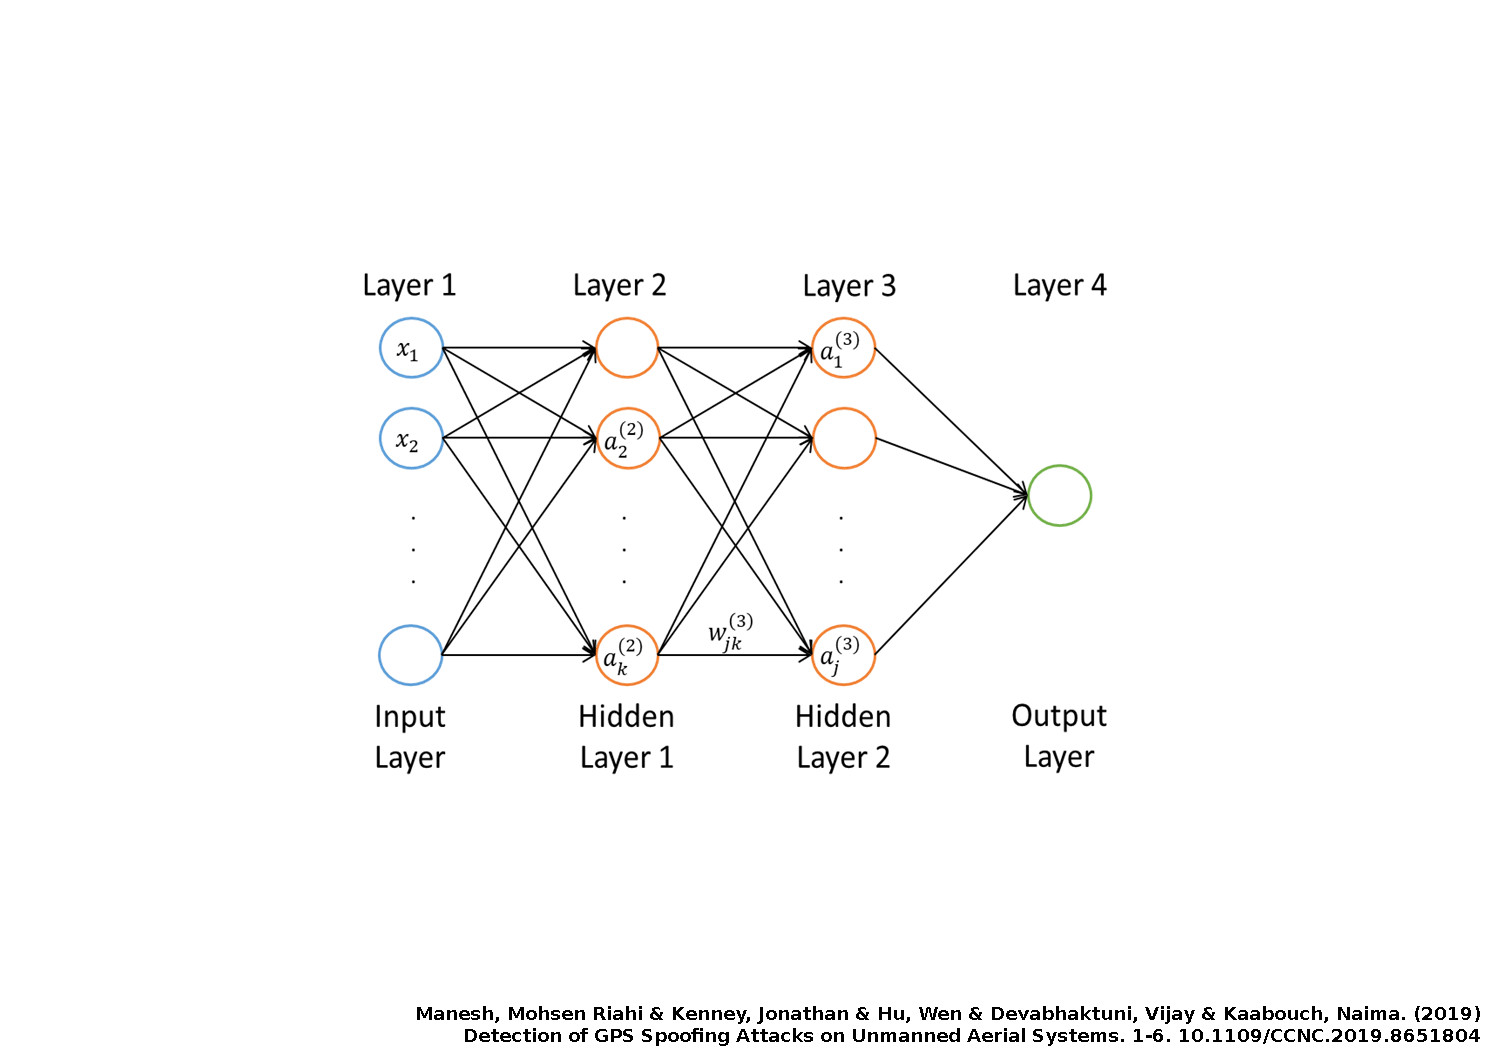
\includegraphics[width=12cm]{5-neuralnetwork.jpg}
}

\frame{
    \frametitle{Sujets de recherche}

    \begin{enumerate}
        \item Représenter graphiquement les grands graphes
        \item Systèmes multi-agents~: exploration collaborative d'un graphe
        \item Recherche de chemins, algorithme A*
        \item Construire la carte d'internet
        \item Marches aléatoires sur les graphes
        \item Graphes planaires et mineurs exclus
        \item Graphes petit-mondes
        \item Réécriture de graphes
        \item Graphes et recommandation "top-N"
        \item Hypergraphes
    \end{enumerate}
}

    \section{Définitions de base}

\frame{
    \frametitle{Graphe}

    \definition{%
        Un graphe est est un couple $\graphedef{}$ avec~:
        \begin{itemize}
            \item $\sommets{}$ un ensemble \enavant{fini} de sommets,
            \item $\arcs{} \subseteq \sommets{}\times\sommets{}$ un ensemble \enavant{fini} d'arrêtes.
        \end{itemize}%
    }

    \uncover<2->{
        \only<1-2>{%
            \exercice{%
                Soit un graphe $\graphedef{}$.
                Quel est, en fonction de $\taille{\sommets{}}$, le nombre maximum d'arrêtes de $\graphe{}$ ?%
            }%
        }

        \only<3->{%
            \proposition{%
                Soit un graphe $\graphedef{}$, on a $\taille{\arcs{}} \leq \taille{\sommets{}}^2$.
            }%
        }
    }

    \uncover<4->{%
        \only<1-4>{%
            \exercice{%
                Soit un graphe $\graphedef{}$ sans sommets isolés.
                Quel est, en fonction de $\taille{\sommets{}}$, le nombre minimum d'arrêtes de $\graphe{}$ ?%
            }%
        }

        \only<5->{%
            \proposition{%
                Soit un graphe $\graphedef{}$ sans sommets isolés, on a $\taille{\arcs{}} \geq \lceil \taille{\sommets{}}/2 \rceil$

            }%
        }
    }
}

\frame{
    \frametitle{Vocabulaire}

    \definition[Successeurs]{%
        Dans un graphe $\graphedef{}$ les successeurs d'un sommet $\sommet{}\in\sommets{}$ sont les sommets $\sommetb{}\in\sommets{}$ tels que $(\sommet{}, \sommetb{})\in\arcs{}$.
    }

    \definition[Prédecesseurs]{%
        Dans un graphe $\graphedef{}$ les prédecesseurs d'un sommet $\sommet{}\in\sommets{}$ sont les sommets $\sommetb{}\in\sommets{}$ tels que $(\sommetb{}, \sommet{})\in\arcs{}$.
    }

    \definition[Graphe complet]{%
        Un graphe $\graphedef{}$ est dit complet si $\arcs{} = \sommets{}\times\sommets{}$.
    }

}

\frame{
    \frametitle{Dessiner les graphes}

    \begin{figure}
        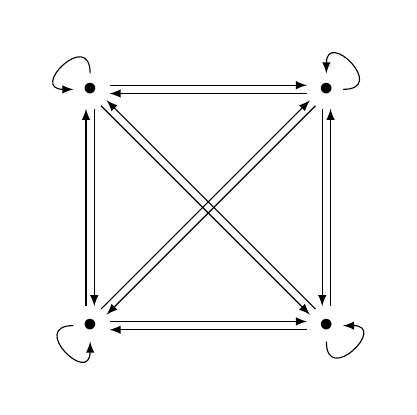
\begin{tikzpicture}
            \node (a) at (0,0) {$\bullet$};
            \node (b) at (3,0) {$\bullet$};
            \node (c) at (0,3) {$\bullet$};
            \node (d) at (3,3) {$\bullet$};

            \shiftdraw{a}{b}{0}{1.5pt};
            \shiftdraw{a}{c}{-1.5pt}{0};
            \shiftdraw{a}{d}{-1pt}{1pt};
            \draw[-latex] (a) to[in=270, out=180, looseness=5] (a);

            \shiftdraw{b}{a}{0}{-1.5pt};
            \shiftdraw{b}{c}{1pt}{1pt};
            \shiftdraw{b}{d}{1.5pt}{0};
            \draw[-latex] (b) to[in=0, out=270, looseness=5] (b);

            \shiftdraw{c}{a}{1.5pt}{0};
            \shiftdraw{c}{b}{-1pt}{-1pt};
            \shiftdraw{c}{d}{0}{1.5pt};
            \draw[-latex] (c) to[in=180, out=90, looseness=5] (c);

            \shiftdraw{d}{a}{1pt}{-1pt};
            \shiftdraw{d}{b}{-1.5pt}{0};
            \shiftdraw{d}{c}{0}{-1.5pt};
            \draw[-latex] (d) to[in=90, out=0, looseness=5] (d);
        \end{tikzpicture}
        \caption{Un graphe complet à 4 sommets}
    \end{figure}
}

\frame{
    \frametitle{Les graphes vus comme des fonctions}

    \definition[À partir des successeurs]{%
        \begin{eqnarray*}
            \graphefunc{} & : & \sommets{} \rightarrow 2^\sommets{} \\
                          &   & \sommet{} \mapsto \{ \sommetb{}~|~(\sommet{}, \sommetb{})\in \arcs{} \}
        \end{eqnarray*}
    }

    \definition[À partir des prédecesseurs]{%
        \begin{eqnarray*}
            \graphefunc{} & : & \sommets{} \rightarrow 2^\sommets{} \\
                          &   & \sommet{} \mapsto \{ \sommetb{}~|~(\sommetb{}, \sommet{})\in \arcs{} \}
        \end{eqnarray*}
    }
}

\frame{
    \frametitle{Les graphes vus comme des matrices}

    \definition[matrice d'adjacence]{%
        Soit $\graphedef{}$ un graphe.
        On pose $n=\taille{\sommets{}}$ et $\sommets{}=\{\sommet{}_1, \dots, \sommet{}_n\}$.
        La matrice d'ajacence de $\graphe{}$ est $\adjmat{\graphe{}}=(\adjmatelem{})_{1\leq i, j \leq n}$ telle que~:
        \begin{eqnarray*}
            \adjmatelem{} = 1 & \textrm{si} & (\sommet{}_i, \sommet{}_j)\in\arcs{} \\
            \adjmatelem{} = 0 & \textrm{sinon} &
        \end{eqnarray*}
    }

    \pause

    \exercice{%
        Donner la matrice d'adjacence du graphe suivant~:

        \begin{center}
        \scalebox{0.6}{%
            \begin{tikzpicture}
                \node (a) at (0,0) {$\sommet{}_3$};
                \node (b) at (3,0) {$\sommet{}_4$};
                \node (c) at (0,3) {$\sommet{}_1$};
                \node (d) at (3,3) {$\sommet{}_2$};
    
                \draw[-latex] (a) to[in=270, out=180, looseness=5] (a);
    
                \shiftdraw{b}{a}{0}{-1.5pt};
    
                \shiftdraw{c}{a}{1.5pt}{0};
                \shiftdraw{c}{d}{0}{1.5pt};
    
                \shiftdraw{d}{b}{-1.5pt}{0};
                \shiftdraw{d}{c}{0}{-1.5pt};
                \draw[-latex] (d) to[in=90, out=0, looseness=5] (d);
            \end{tikzpicture}
        }
        \end{center}
    }
}

\frame{
    \frametitle{Les graphes vus comme des matrices, suite}

    \notation{%
        Soit $\graphedef{}$ un graphe et soit $\arc{} = (\sommet{}, \sommetb{})\in\arcs{}$ une arrête, on note $\sommet{} = \arcdepuis{\arc{}}$ et $\sommetb{} = \arcvers{\arc{}}$.
    }

    \definition[matrice d'incidence]{%
        Soit $\graphedef{}$ un graphe.
        On pose $n=\taille{\sommets{}}$ et $\sommets{}=\{\sommet{}_1, \dots, \sommet{}_n\}$.
        De même, on pose $m=\taille{\arcs{}}$ et $\arcs{}=\{\arc{}_1, \dots, \arc{}_m\}$.
        La matrice d'incidence de $\graphe{}$ est la matrice $\incmat{\graphe{}} = (\incmatelem{})_{1\leq i\leq n, 1\leq j\leq m}$ telle que~:
        \begin{eqnarray*}
            \incmatelem{} = 1 & \textrm{si} & \arcdepuis{\arc{}_j} = \sommet{}_i \\
            \incmatelem{} = -1 & \textrm{si} & \arcvers{\arc{}_j} = \sommet{}_i \\
            \incmatelem{} = 0 & sinon &
        \end{eqnarray*}
    }
}

\frame{
    \frametitle{Les graphes vus comme des matrices, suite, suite}

    \exercice{%
        Donner la matrice d'incidence du graphe suivant~:
        \begin{center}
            \scalebox{0.8}{%
                \begin{tikzpicture}
                    \node (a) at (0,0) {$\sommet{}_3$};
                    \node (b) at (3,0) {$\sommet{}_4$};
                    \node (c) at (0,3) {$\sommet{}_1$};
                    \node (d) at (3,3) {$\sommet{}_2$};
        
                    \node (tmp) at (1.5,3.3) {$\arc{}_1$};
                    \node (tmp) at (1.5,2.7) {$\arc{}_2$};
                    \node (tmp) at (-0.3,1.5) {$\arc{}_3$};
                    \node (tmp) at (3.3,1.5) {$\arc{}_4$};
                    \node (tmp) at (1.5,-0.3) {$\arc{}_5$};

                    \shiftdraw{b}{a}{0}{-1.5pt};
        
                    \shiftdraw{c}{a}{1.5pt}{0};
                    \shiftdraw{c}{d}{0}{1.5pt};
        
                    \shiftdraw{d}{b}{-1.5pt}{0};
                    \shiftdraw{d}{c}{0}{-1.5pt};
                \end{tikzpicture}
            }
        \end{center}
    }

    \pause

    \remarque{%
        La représentation en matrice d'incidence ne permet pas d'avoir des arcs $\arc{}$ tels que $\arcdepuis{\arc{}} = \arcvers{\arc{}}$.
    }
}

\frame{
    \frametitle{Structures de données classiques}

    Les structures de données qu'on utilise le plus souvent pour représenter les graphes sont les suivantes~:
    \begin{itemize}
        \item matrice d'adjacence
        \item listes de successeurs
        \item listes de prédécesseurs
    \end{itemize}

    \pause

    \exercice{%
        Donner la représentation en listes de successeurs et en listes de prédecesseurs du graphe dont on a précédement donné la matrice d'adjacence.
    }

    \exercice{%
        Proposer un algorithme qui permet d'obtenir une représentation en listes de successeurs à partir d'une représentation en matrice d'adjacence.
    }
}

\frame{
    \frametitle{Voisins}

    \definition[prédecesseurs]{%
        Dans un graphe $\graphedef{}$ l'ensemble des prédecesseurs d'un sommet $\sommet{}\in\sommets{}$ est noté~:
        $$\pre{\sommet{}} = \{\sommetb{}~|~(\sommetb{},\sommet{}\in\arcs{})\}$$
    }

    \definition[successeurs]{%
        Dans un graphe $\graphedef{}$ l'ensemble des successeurs d'un sommet $\sommet{}\in\sommets{}$ est noté~:
        $$\suc{\sommet{}} = \{\sommetb{}~|~(\sommet{},\sommetb{}\in\arcs{})\}$$
    }

    \definition[voisins d'un sommet]{%
        Soit un graphe $\graphedef{}$, soit un sommet $\sommet{}\in\sommets{}$, on appelle voisins de $\sommet{}$ les sommets qui sont soit des prédécesseurs soit des successeurs de $\sommet{}$, c'est-à-dire les sommets de l'ensemble $\voisins{\sommet{}} = \pre{\sommet{}}\cup\suc{\sommet{}}$.
    }
}

\frame{
    \frametitle{Degré}

    \definition[degré entrant]{%
        Soit un graphe $\graphedef{}$, soit un sommet $\sommet{}\in\sommets{}$, le degré entrant de $\sommet{}$ est $\dege{\sommet{}} = \taille{\pre{\sommet{}}}$.
    }

    \definition[degré sortant]{%
        Soit un graphe $\graphedef{}$, soit un sommet $\sommet{}\in\sommets{}$, le degré sortant de $\sommet{}$ est $\degs{\sommet{}} = \taille{\suc{\sommet{}}}$.
    }

    \definition[degré d'un sommet]{%
        Soit un graphe $\graphedef{}$, soit un sommet $\sommet{}\in\sommets{}$, le degré de $\sommet{}$ est $\degre{\sommet{}} = \dege{\sommet{}} + \degs{\sommet{}}$.
    }

    \definition[degré d'un graphe]{%
        Soit un graphe $\graphedef{}$, le degré de $\graphe{}$ est $\degre{\graphe{}} = \max_{\sommet{}\in\sommets{}} \degre{\sommet{}}$
    }
}

\frame{
    \frametitle{Graphes et relations binaires}

    On peut représenter une relation binaire $\relation{}$ sur un ensemble fini $\ensemble{}$ par un graphe $\graphedef{}$ dont
    \begin{itemize}
        \item les sommets sont les éléments de l'ensemble~: $\sommets{} = \ensemble{}$,
        \item les arrêtes représentent la relation~: $(x, y) \in \arcs{} \Leftrightarrow x\relation{}y$.
    \end{itemize}

    Un certain nombre de caractéristiques de la relation peuvent alors se repérer visuellement sur le graphe.

    \begin{columns}
        \begin{column}{5.5cm}
            \begin{block}{Réflexivité~: $\forall x, x\relation{}x$}
                \begin{center}
                    \begin{tikzpicture}
                        \node (a) at (0,0) {$x$};
                        \draw[-latex] (a) to[in=90, out=0, looseness=5] (a);
                    \end{tikzpicture}
                \end{center}
            \end{block}
            \begin{block}{Symétrie~: $\forall x, y, x\relation{}y \Rightarrow y\relation{}x$}
                \begin{center}
                    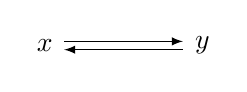
\begin{tikzpicture}
                        \node (a) at (0,0) {$x$};
                        \node (b) at (2,0) {$y$};
                        \shiftdraw{a}{b}{0}{1.5pt};
                        \shiftdraw{b}{a}{0}{-1.5pt};
                    \end{tikzpicture}
                \end{center}
            \end{block}
        \end{column}
        \begin{column}{5.5cm}
            \begin{block}{Transitivité~: $\forall x, y, z, x\relation{}y \textrm{ et } y\relation{}z \Rightarrow x\relation{}z$}
                \begin{center}
                    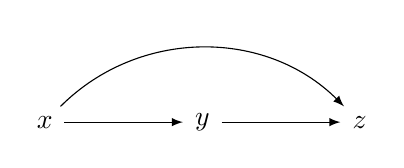
\begin{tikzpicture}
                        \node (a) at (0,0) {$x$};
                        \node (b) at (2,0) {$y$};
                        \node (c) at (4,0) {$z$};
                        \shiftdraw{a}{b}{0}{0};
                        \shiftdraw{b}{c}{0}{0};
                        \draw[-latex] (a) to[out=45, in=135] (c);
                    \end{tikzpicture}
                \end{center}
            \end{block}
        \end{column}
    \end{columns}
}

\frame{
    \frametitle{Graphes et relations binaires, suite}

    \exercice[relation d'équivalence]{%
        Comment peut-on caractériser le graphe représentant une relation d'équivalence (réflexive, symétrique et transitive) ?
    }

    \exercice[antisymmétrie]{%
        Une relation $\relation{}$ est dite antisymétrique si $\forall x, y, x\relation{}y \textrm{ et } y\relation{}x \Rightarrow x = y$.
        Comment cela se traduit-il visuellement dans un graphe ?
    }

    \exercice[relation d'ordre]{%
        Coment peut-on caractériser le graphe représentant une relation d'ordre (réflexive, antisymétrique et transitive)
    }
}

    \section{Graphe des chemins}

\frame{
    \frametitle{Chemins}

    \definition[chemin]{%
        Soit $\graphedef{}$ un graphe.
        Un chemin (de $\sommet{}_0$ à $\sommet{}_n$) de $\graphe{}$ est une suite $\sommet{}_0\sommet{}_1 \dots \sommet{}_n$ de sommets telle que $\forall i\in[0,n[, (\sommet{}_i, \sommet{}_{i+1})\in \arcs{}$.
    }

    \notation[chemin]{%
        S'il en existe, on peut noter $\sommet{} \cheminvers \sommetb{}$ un chemin quelconque de $\sommet{}$ à $\sommetb{}$ dans un graphe $\graphe{}$.
    }

    \definition[longueur d'un chemin]{%
        Soit $\chemin{} = \sommet{}_0\sommet{}_1\dots\sommet{}_n$ un chemin du graphe $\graphe$.
        La longueur de $\chemin{}$ est le nombre d'arrêtes de $\chemin{}$~:
        $$\taille{\chemin{}} = \taille{\{(\sommet{}_0,\sommet{}_1), (\sommet{}_1,\sommet{}_2), \dots, (\sommet{}_{n-1},\sommet{}_n)\}} = n.$$
    }
}

\frame{
    \frametitle{Graphe des chemins}

    \definition[graphe des chemins]{%
        Soit $\graphedef{}$ un graphe, le graphe $\graphechemdef$ tel que~:
        \begin{eqnarray*}
            \sommetschem & = & \sommets \\
            \arcschem & = & \{(\sommet{}, \sommetb{})~|~\exists \textrm{ chemin de } \sommet{} \textrm{ à } \sommetb{} \textrm{ dans } \graphe{}\}
        \end{eqnarray*}
        s'appelle le graphe des chemins de $\graphe{}$.
    }

    \pause

    \exercice{%
        Donner le graphe des chemins du graphe suivant~:
        \begin{center}
            \scalebox{0.6}{
            \begin{tikzpicture}
                \node (a) at (0,0) {$\bullet$};
                \node (b) at (3,0) {$\bullet$};
                \node (c) at (0,3) {$\bullet$};
                \node (d) at (3,3) {$\bullet$};

                \shiftdraw{a}{b}{0}{1.5pt};
                \draw[-latex] (a) to[in=270, out=180, looseness=5] (a);

                \shiftdraw{b}{d}{1.5pt}{0};

                \shiftdraw{c}{d}{0}{1.5pt};

                \shiftdraw{d}{c}{0}{-1.5pt};
            \end{tikzpicture}
            }
        \end{center}
    }
}

\frame{
    \frametitle{Objectif de cette partie}

    On se donne un graphe $\graphe$ et on souhaite savoir calculer (efficacement) son graphe des chemins $\graphechem$.
}

\frame{
    \frametitle{Propriétés du graphe des chemins}

    \proposition[$\graphechem$ est transitif]{%
        Soit $\graphedef{}$ un graphe et soit $\graphechemdef$ son graphe des chemins.
        Quels que soient $\sommet{}, \sommetb{}, \sommetc{} \in \sommetschem{}$ on a $$(\sommet{}, \sommetb{}) \in \arcschem{} \textrm{ et } (\sommetb{}, \sommetc{}) \in \arcschem \Rightarrow (\sommet{}, \sommetc{}) \in \arcschem{}.$$
    }

    \exercice{%
        Prouver la proposition.
    }
}

\frame{
    \frametitle{Propriétés du graphe des chemins, suite}

    \definition{%
        Soient $\graphe{}_1$ et $\graphe{}_2$ des graphes, on note $\graphe{}_1\infgraphe{}\graphe{}_2$ si $\sommets{}_1 \subseteq \sommets{}_2$ et $\arcs{}_1\subseteq\arcs{}_2$.
    }

    \pause

    \begin{columns}
        \begin{column}{5.5cm}
            \proposition{%
                $\infgraphe{}$ est une relation d'ordre.
            }
        \end{column}
        \begin{column}{5.5cm}
            \exercice{%
                Prouver la proposition.
            }
        \end{column}
    \end{columns}

    \pause

    \proposition{%
        Étant donné un graphe $\graphe{}$, son graphe des chemins $\graphechem{}$ est le plus petit graphe (pour la relation $\infgraphe{}$) transitif qui contient $\graphe{}$~:
        $$\forall H, \graphe{} \infgraphe{} H \textrm{ et } H \textrm{ transifif } \Rightarrow \graphechem{} \infgraphe{} H$$
    }

    \exercice{%
        Prouver la proposition.
    }
}

\subsection{Opérations sur les graphes}

\frame{
    \frametitle{Union}

    À partir de maintenant, on considère que tous les graphes ont le même ensemble $\sommets{}$ de sommets.

    \definition[union de graphes]{%
        Soient $\graphe{}_1=(\sommets{}, \arcs{}_1)$ et $\graphe{}_2=(\sommets{}, \arcs{}_2)$ deux graphes.
        L'union de $\graphe{}_1$ et $\graphe{}_2$ est le graphe $\graphe{}_1\uniong{}\graphe{}_2 = (\sommets{}, \arcs{}_1\cup\arcs{}_2)$.
    }

    \pause

    \begin{columns}
        \begin{column}{6.5cm}
            \proposition[associativité]{%
                $\graphe{}_1\uniong{}(\graphe{}_2\uniong{}\graphe{}_3) = (\graphe{}_1\uniong{}\graphe{}_2)\uniong{}\graphe{}_3$%
            }
        \end{column}
        \begin{column}{4.5cm}
            \exercice{Le prouver}
        \end{column}
    \end{columns}

    \pause

    \begin{columns}
        \begin{column}{6.5cm}
            \proposition[élément neutre]{%
                $\emptyset = (V, \emptyset), \graphe{}\uniong{}\emptyset = \emptyset\uniong{}\graphe{} = \graphe{}$ 
            }
        \end{column}
        \begin{column}{4.5cm}
            \exercice{Le prouver}
        \end{column}
    \end{columns}

    \pause

    \begin{columns}
        \begin{column}{6.5cm}
            \proposition[commutativité]{%
                $\emptyset = (V, \emptyset), \graphe{}\uniong{}\emptyset = \emptyset\uniong{}\graphe{} = \graphe{}$ 
            }
        \end{column}
        \begin{column}{4.5cm}
            \exercice{Le prouver}
        \end{column}
    \end{columns}
}

\frame{
    \frametitle{Représentation matricielle}

    \proposition{%
        Soit $\graphe{}_1$ un graphe représenté par la matrice d'adjacence $\adjmat{\graphe{}_1}=(a_{ij}^1)$ et soit $\graphe{}_2$ un graphe représenté par la matrice d'adjacence $\adjmat{\graphe{}_2} = (a_{ij}^2)$.
        Soit $\graphe{} = \graphe{}_1\uniong{}\graphe{}_2$ et soit $\adjmat{\graphe{}} = (\adjmatelem{})$ sa matrice d'adjacence.
        On a~: $$\adjmatelem{} = a_{ij}^1 \vee a_{ij}^2.$$
    }

    \exercice{Le prouver}

    \pause
    \vfill

    Conséquence~: on peut voir l'union des graphes comme une \enavant{somme de} leurs \enavant{matrices} d'adjacence.
}

\frame{
    \frametitle{Algorithme pour calculer une union de graphes}

    \begin{center}
        \begin{minipage}{8cm}
            \begin{algorithmic}
                \In{$\graphe{}_1 = (\sommets{}, \arcs{}_1)$, $\graphe{}_2 = (\sommets{}, \arcs{}_2)$}
                \Out{$\graphedef{} = \graphe{}_1\uniong\graphe{}_2$}
                \State $\arcs{} = \emptyset$
                \ForAll{$\sommet{} \in \sommets{}$} 
                    \ForAll{$\sommetb{} \in \sommets{}$}
                        \If{$(\sommet{}, \sommetb{})\in \arcs{}_1$ {\bf or} $(\sommet{}, \sommetb{})\in \arcs{}_2$}
                            \State $\arcs{} = \arcs{}\cup \{(\sommet{}, \sommetb{})\}$
                        \EndIf
                    \EndFor
                \EndFor 
            \end{algorithmic}
        \end{minipage}
    \end{center}

    \vspace{1cm}
    \pause

    \exercice{%
        Donner la complexité de cet algorithme.
    }
}

\frame{
    \frametitle{Composition}

    \definition[composition de graphes]{%
    Soient $\graphe{}_1=(\sommets{}, \arcs{}_1)$ et $\graphe{}_2=(\sommets{}, \arcs{}_2)$ deux graphes.
    La composition de $\graphe{}_1$ et $\graphe{}_2$ est le graphe $\graphe{}_1\compog{}\graphe{}_2 = (\sommets{}, \arcs{})$ tel que~:
    $$E = \{(\sommet{}, \sommetb{})~|~\exists\sommetc{}, (\sommet{}, \sommetc{})\in\arcs{}_1 \textrm{ et } (\sommetc{}, \sommetb{})\in\arcs{}_2\}.$$
    }

    \pause

    \begin{columns}
        \begin{column}{6.5cm}
            \proposition[associativité]{%
                $\graphe{}_1\compog{}(\graphe{}_2\compog{}\graphe{}_3) = (\graphe{}_1\compog{}\graphe{}_2)\compog{}\graphe{}_3$%
            }
        \end{column}
        \begin{column}{4.5cm}
            \exercice{Le prouver}
        \end{column}
    \end{columns}

    \pause

    \begin{columns}
        \begin{column}{6.5cm}
            \proposition[élément neutre]{%
                $(\sommets{}, \{(\sommet{}, \sommet{})~|~ \sommet{}\in\sommets{}\})$ 
            }
        \end{column}
        \begin{column}{4.5cm}
            \exercice{Le prouver}
        \end{column}
    \end{columns}

    \pause

    \begin{columns}
        \begin{column}{6.5cm}
            \proposition[commutativité]{%
                La composition n'est pas commutative. 
            }
        \end{column}
        \begin{column}{4.5cm}
            \exercice{Le prouver}
        \end{column}
    \end{columns}
}

\frame{
    \frametitle{Composition, suite}

    \proposition[distributivité]{%
        La composition est distributive par rapport à l'union~:
        $$(\graphe{}_1\uniong{}\graphe{}_2)\compog{}\graphe{}_3 = (\graphe{}_1\compog{}\graphe{}_3)\uniong{}(\graphe{}_2\compog{}\graphe{}_3)$$
        $$\graphe{}_1\compog{}(\graphe{}_2\uniong{}\graphe{}_3) = (\graphe{}_1\compog{}\graphe{}_2)\uniong{}(\graphe{}_1\compog{}\graphe{}_3)$$
    }

    \exercice{Le prouver}
}

\frame{
    \frametitle{Représentation matricielle}

    \proposition{%
        Soit $\graphe{}_1$ un graphe représenté par la matrice d'adjacence $\adjmat{\graphe{}_1}=(a_{ij}^1)$ et soit $\graphe{}_2$ un graphe représenté par la matrice d'adjacence $\adjmat{\graphe{}_2} = (a_{ij}^2)$.
        Soit $\graphe{} = \graphe{}_1\compog{}\graphe{}_2$ et soit $\adjmat{\graphe{}} = (\adjmatelem{})$ sa matrice d'adjacence.
        On a~: $$\adjmatelem{} = \bigvee_{k=1}^{\taille{\sommets{}}} a_{ik}^1 \wedge a_{kj}^2.$$
    }

    \exercice{Le prouver}

    \pause
    \vfill

    Conséquence~: on peut voir l'union des graphes comme un \enavant{produit de} leurs \enavant{matrices} d'adjacence.
}

\frame{
    \frametitle{Algorithme pour calculer une composition de graphes}

    \begin{center}
        \begin{minipage}{9cm}
            \begin{algorithmic}
                \In{$\graphe{}_1 = (\sommets{}, \arcs{}_1)$, $\graphe{}_2 = (\sommets{}, \arcs{}_2)$}
                \Out{$\graphedef{} = \graphe{}_1\compog\graphe{}_2$}
                \State $\arcs{} = \emptyset$
                \ForAll{$\sommet{} \in \sommets{}$} 
                    \ForAll{$\sommetc{} \in \sommets{}$}
                        \ForAll{$\sommetb{} \in \sommets{}$}
                            \If{$(\sommet{}, \sommetb{})\in \arcs{}_1$ {\bf and} $(\sommetb{}, \sommetc{})\in \arcs{}_2$}
                                \State $\arcs{} = \arcs{}\cup \{(\sommet{}, \sommetc{})\}$
                            \EndIf
                        \EndFor
                    \EndFor
                \EndFor 
            \end{algorithmic}
        \end{minipage}
    \end{center}

    \pause

    \exercice{%
        Donner la complexité de cet algorithme.
    }

    \pause

    \exercice{%
        Proposer une optimisation simple permettant souvent de réduire le nombre de tours de la boucle interne.
    }
}

\subsection{Algorithme des puissances}

\frame{
    \frametitle{Exercice introductif}

    \exercice{%
        \begin{columns}
            \begin{column}{6cm}
                On considère le graphe $\graphe{}$ suivant~:
                
                ~
                
                \begin{tikzpicture}
                    \node (a) at (0,0) {$\sommet{}_3$};
                    \node (b) at (3,0) {$\sommet{}_4$};
                    \node (c) at (0,3) {$\sommet{}_1$};
                    \node (d) at (3,3) {$\sommet{}_2$};

                    \node (tmp) at (1.5, 3.3) {$\arc{}_1$};
                    \node (tmp) at (3.3, 1.5) {$\arc{}_3$};
                    \node (tmp) at (1.2, 1.8) {$\arc{}_2$};
                    \node (tmp) at (-0.7, -0.7) {$\arc{}_4$};

                    \shiftdraw{a}{d}{-1pt}{1pt};
                    \draw[-latex] (a) to[in=270, out=180, looseness=5] (a);

                    \shiftdraw{c}{d}{0}{1.5pt};

                    \shiftdraw{d}{b}{-1.5pt}{0};
                \end{tikzpicture}
            \end{column}
            \begin{column}{5cm}
                \begin{itemize}
                    \item Calculer $\graphe{}\compog{}\graphe{}$.
                    \item Quel est le lien entre les arrêtes de $\graphe{}\compog{}\graphe{}$ et les chemins de $\graphe{}$ ?
                    \item Calculer $\graphe{}\uniong{}(\graphe{}\compog{}\graphe{})$.
                    \item Quel est le lien entre les arrêtes de $\graphe{}\uniong{}(\graphe{}\compog{}\graphe{})$ et les chemins de $\graphe{}$ ?
                \end{itemize}
            \end{column}
        \end{columns}
    }
}

\frame{
    \frametitle{Une suite intéressante}

    \definition{%
        Étant donné un graphe $\graphe{}$, soit la suite $\suitepuiss{}$ définie par~:
        \begin{eqnarray*}
            \suiteelem{1} & = & \graphe{} \\
            \suiteelem{n} & = & \suiteelem{n-1}\compog{}\graphe{}
        \end{eqnarray*}
    }

    \pause

    \proposition{%
        Le n-ième terme $\suiteelem{n} = (\sommets{}, \arcs{}_n)$ de cette suite est tel que~:
        $$\arcs{}_n = \{(\sommet{}, \sommetb{})~|~\exists \textrm{ chemin de longueur } n \textrm{ de } \sommet{} \textrm{ à } \sommetb{} \textrm{ dans } \graphe{}\}$$
    }

    \exercice{%
        Prouver la proposition (on peut le faire par récurrence sur la longueur des chemins/le numéro du terme de la suite).
    }
}

\frame{
    \frametitle{Une suite intéressante, suite}

    \proposition{%
        Pour tout graphe $\graphedef{}$ on a~:
        $$\graphechem{} = \underset{n=1~~}{\overset{\taille{\arcs{}}~~}{\uniong{}}} \suiteelem{n} = \underset{n=1~~}{\overset{\taille{\sommets{}}~~}{\uniong{}}} \suiteelem{n}$$
    }

    \exercice{%
        Prouver la proposition (cela revient essentiellement à prouver que s'il y a un chemin de $\sommet{}$ à $\sommetb{}$ dans $\graphe{}$ alors il en existe un de longueur $\leq \taille{\arcs{}}$ et un de longueur $\leq \taille{\sommets{}}$).
    }

    \pause

    \begin{center}
        Cette proposition donne une méthode de calcul de $\graphechem{}$ à partir de $\graphe{}$.
    \end{center}

    \pause

    \exercice{%
        Soit un graphe $\graphedef{}$.
        Combien de compositions et d'unions fait-on pour calculer $\graphechem{}$ avec cette méthode ?
        (on peut noter $n = \min(\taille{\sommets{}}, \taille{\arcs{}})$.)%
    }
}

\frame{
    \frametitle{Une suite encore plus intéressante}

    \definition[Schéma de Hörner]{%
        Étant donné un graphe $\graphe{}$, on appelle schéma de Hörner la suite $\horner{}$ définie par~:
        \begin{eqnarray*}
            \hornerelem{1} & = & \graphe{} \\
            \hornerelem{n} & = & (\hornerelem{n-1} \compog{} \graphe{}) \uniong{} \graphe{}
        \end{eqnarray*}
    }

    \proposition{%
        $$\hornerelem{\taille{\sommets{}}} = \hornerelem{\taille{\arcs{}}} = \graphechem{}$$
    }

    \pause

    \exercice{%
        Prouver la proposition. 
        On pourra pour cela montrer par récurrence sur $n$ que $\hornerelem{n} = \uniong{}_{k=1}^n \suiteelem{k}$ pour tout $n\geq 1$.
    }
}

\frame{
    \frametitle{Une suite encore plus intéressante, suite}

    \exercice{%
        Soit un graphe $\graphedef{}$.
        Combien d'unions et de compositions fait-on pour calculer $\graphechem{}$ à l'aide du schéma de Hörner ?
    }

    \pause

    Le schéma de Hörner est donc plus efficace que le simple calcul de la suite précédente.
    On peut encore améliorer cela à partir de la proposition suivante.
    On aboutit alors à un algorithme qu'on appelle \enavant{algorithme des puissances}.

    \proposition{%
        Si $\hornerelem{p} = \hornerelem{p+1}$ alors $\forall q \geq p, \hornerelem{q} = \hornerelem{p}$.
    }

    \pause

    \exercice{%
        Prouver la proposition (par récurrence).
    }
}

\frame{
    \frametitle{Algorithme des puissances}

    \begin{center}
        \begin{minipage}{6cm}
            \begin{algorithmic}
                \In{$\graphedef{}$}
                \Out{$\hornerelem{} = \graphechem{}$}
                \State $\hornerelem{} = \graphe{}$
                \State $\hornerelem{t} = (\sommets{}, \emptyset)$
                \While{$\hornerelem{} \neq \hornerelem{t}$} 
                    \State $\hornerelem{t} = \hornerelem{}$
                    \State $\hornerelem{} = (\hornerelem{} \compog{} \graphe{}) \uniong{} \graphe{}$
                \EndWhile
            \end{algorithmic}
        \end{minipage}
    \end{center}

    \exercice{%
        Quelle est la complexité de l'algorithme des puissances en fonction de $n=\min(\taille{\sommets{}}, \taille{\arcs{}})$
    }
}

\frame{
    \frametitle{Algorithme des puissances, suite}

    \remarque{%
        Le véritable temps d'exécution de cet algorithme varie fortement en fonction du graphe considéré~: il peut s'arrêter très vite ou, au contraire, effectuer son maximum de $\min(\taille{\sommets{}}, \taille{\arcs{}})$ itérations.
    }

    \exercice{%
        Proposer un graphe (avec un ensemble de sommets et un ensemble d'arcs non vides) $\graphe{}_{min}$ tel qu'on ne fasse qu'une seule itération de la boucle de l'algorithme des puissances pour calculer son graphe des chemins.
    }

    \exercice{%
        Proposer un graphe $\graphe{}_{max}$ tel qu'on atteigne les $\min(\taille{\sommets{}}, \taille{\arcs{}})$ itérations pour calculer le graphe des chemins de $\graphe{}_{max}$ avec l'algorithme des puissances.
    }
}

\subsection{Algorithme de Roy-Warshall}

\frame{
    \frametitle{Idée générale}

    On va présenter ici un algorithme dont la complexité est meilleure que celle de l'algorithme des puissances~: de l'ordre de $\taille{\sommets{}}^3$.

    \pause

    \vfill{}

    Pour toute cette partie on travail sur un graphe $\graphedef$ et on ordonne (arbitrairement) les sommets de $\sommets{}$.

    \notation{%
        On pose $\sommets{} = \{\sommet{}_1, \sommet{}_2, \dots, \sommet{}_n\}$ et $\sommet{}_1 < \sommet{}_2 < \dots < \sommet{}_n$.%
    }

    \notation{%
        On note $\sommets{}_i = \{\sommet{}_1, \sommet{}_2, \dots, \sommet{}_i\}$, l'ensemble des sommets qui arrivent avant $\sommet{}_i$ selon l'ordre choisi.%
    }

    \proposition{%
        $$\emptyset \subset \sommets{}_0 \subset \sommets{}_1 \subset \dots \subset \sommets{}_n = \sommets{}$$%
    }
}

\frame{
    \frametitle{Idée générale, suite}

    On s'intéresse aux chemins constitués uniquement des sommets d'un sous ensemble $\sommets{}_i$ donné, au lieu de s'intéresser aux chemins d'une longueur donnée comme dans l'algorithme des puissances.

    \notation{%
        \begin{eqnarray*}
            \roy{i} = \{(\sommet{}, \sommetb{}) & | & \exists \sommet\sommet{}_{i_1}\sommet{}_{i_2}\dots\sommet{}_{i_k}\sommetb{} \textrm{ un chemin de } \graphe{} \\
                                               &   & \textrm{ tel que } \{\sommet{}_{i_1}, \sommet{}_{i_2}, \dots, \sommet{}_{i_k}\} \in \sommets{}_i\}
        \end{eqnarray*}%
    }

    \pause

    \proposition{%
        $$\forall i\geq 0, \roy{i} \subseteq \roy{i+1}$$
    }

    \exercice{%
        Prouver la proposition.
    }
}

\frame{
    \frametitle{Idée générale, suite, suite}

    \proposition{%
        $$\forall i\geq 0, \arcs{} \subseteq \roy{i}$$
    }

    \exercice{%
        Prouver la proposition.
    }

    \pause

    \proposition{%
        $$\graphechem{} = (\sommets{}, \roy{\taille{\sommets{}}}))$$
    }

    \exercice{%
        Prouver la proposition.
    }
}

\frame{
    \frametitle{Propriété fondamentale}

    \proposition{%
        $$\forall i\geq 0, \roy{i+1} = \roy{i} \cup \{ (\sommet{}, \sommetb{}) ~|~ (\sommet{}, \sommet{}_{i+1}) \in \roy{i} \textrm{ et} (\sommet{}_{i+1}, \sommetb{}) \in \roy{i}\}$$
    }

    \pause

    Pour faire la preuve on passe par le lemme suivant.

    \definition[chemin élémentaire]{%
        Soit $\chemin{} = \sommet{}_1\sommet{}_2\dots\sommet{}_n$ un chemin d'un graphe $\graphe{}$.
        Si $\forall (i,j) \neq (1,n), \sommet{}_i\neq\sommet{}_j$ alors $\chemin{}$ est dit élémentaire.
    }

    \proposition[lemme pour la preuve de la proposition précédente]{%
        Soit $\graphe{}$ un graphe, s'il existe un chemin de $\sommet{}$ à $\sommetb{}$ dans $\graphe{}$ alors il existe un chemin élémentaire qui n'utilise pas plus de sommets de $\sommet{}$ à $\sommetb{}$ dans $\graphe{}$.
    }

    \pause

    \exercice{%
        Prouver le lemme.
    }
}

\frame{
    \frametitle{Vers l'algorithme de Roy-Warshall}

    \exercice{%
        À l'aide du lemme, prouver la proposition précédente puis déduire de celle-ci un algorithme pour calculer $\graphechem$ à partir des $\roy{i}$.
    }

    \pause

    \vfill{}

    \begin{center}
        \begin{minipage}{9cm}
            \begin{algorithmic}
                \In{$\graphedef{}$}
                \Out{$(\sommets{}, \roy{\taille{\sommets{}}}) = \graphechem{}$}
                \State $\roy{0} = \arcs{}$
                \For{$i = 1$ {\bf to} $\taille{\sommets}$}
                    \State $\roy(i) = \roy{i-1}$
                    \ForAll{$\sommet{} \in \sommets{}$}
                        \ForAll{$\sommetb{} \in \sommets{}$}
                            \If{$(\sommet{}, \sommet{}_i) \in \roy{i-1}$ {\bf and} $(\sommet{}_i, \sommetb{}) \in \roy{i-1}$}
                                \State $\roy{i} = \roy{i} \cup \{(\sommet{}, \sommetb{})\}$
                            \EndIf
                        \EndFor
                    \EndFor
                \EndFor
            \end{algorithmic}
        \end{minipage}
    \end{center}
}

\subsection{Retrouver les chemins}

\frame{}

    \section{Parcours de graphes}

\frame{
    \frametitle{Ce qu'on veut faire}

    À partir d'un sommet $\sommet{}_0$ connu, déterminer les sommets d'un graphe $\graphe{}$ qui sont \enavant{atteignables} depuis $\sommet{}_0$, c'est-à-dire les sommets $\sommet{}$ tels qu'il existe un chemin de $\sommet{}_0$ à $\sommet{}$ dans $\graphe{}$. 
}

\subsection{Schéma générique}

\frame{
    \frametitle{Schéma générique d'exploration}

    \begin{columns}
        \begin{column}{5.5cm}
            \begin{description}
                \item[État initial~:] $\sommet{}_0$ est marqué\\ (c'est le seul)
                \item[Règle d'évolution~:] si $\sommet{}$ marqué et $\sommetb{}$ pas marqué et $(\sommet{}, \sommetb{})\in\arcs{}$, alors marquer $\sommetb{}$
                \item[État final~:]  plus aucune règle ne s'applique
            \end{description}
        \end{column}
        \begin{column}{5cm}
            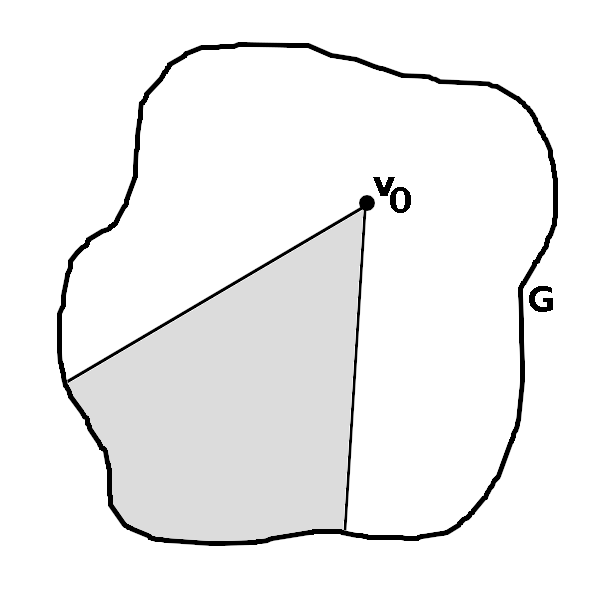
\includegraphics{schemagen.png}
        \end{column}
    \end{columns}
}

\frame{
    \frametitle{Propriétés}

    \proposition[sûreté]{%
        Si $\sommet{}$ est marqué alors il est atteignable depuis $\sommet{}_0$ (il existe un chemin de $\sommet{}_0$ à $\sommet{}$ dans $\graphe{}$)
    }

    \proposition[vivacité/terminaison]{%
        En appliquant la règle d'évolution en fini toujours par atteindre un état dans lequel il n'est plus possible de l'appliquer.
    }

    \proposition[complétude]{%
        Dans un état final, tout sommet atteignable depuis $\sommet{}_0$ est marqué.
    }

    \pause

    \exercice{%
        Prouver ces trois propositions.
    }
}

\subsection{Algorithme de parcours}

\frame{
    \frametitle{Le tas, une structure de données générique}

    \begin{block}{Interface}
        \begin{description}
            \item[init] créer un tas vide
            \item[ajouter] ajouter un élément dans le tas
            \item[observer] obtenir un élément du tas 
            \item[extraire] enlever un élément du tas
            \item[estVide] vérifier s'il reste des éléments dans le tas 
        \end{description}
    \end{block}

    Si le tas n'a pas changé entre observer et extraire, \enavant{l'élément qui est enlevé du tas doit être celui qui avait été obtenu}.

    \begin{exampleblock}{Exemple}
        \begin{center}
            \begin{minipage}{5cm}
                \begin{algorithmic}
                    \State $t = init()$
                    \State $t.ajouter(5)$
                    \If{$!t.estVide()$}
                        \State $v = t.observer()$
                        \State $t.extraire()$
                    \EndIf
                \end{algorithmic}
            \end{minipage}
        \end{center}
    \end{exampleblock}
}

\frame{
    \frametitle{Algorithme de parcours générique}

    \begin{columns}
        \begin{column}{7cm}
            \begin{center}
                \begin{minipage}{7cm}
                    \begin{algorithmic}
                        \In{$\graphedef{}$, $\sommet{}_0\in\sommets{}$}
                        \Out{???}
                        \State $t = init()$
                        \State $t.ajouter(\sommet{}_0)$
                        \State marquer $\sommet{}_0$
                        \While{$!t.estVide()$}
                            \State $v = t.observer()$
                            \If{$\exists (\sommet{}, \sommetb{})\in \arcs{}$, $\sommetb{}$ non marqué}
                                \State $t.ajouter(\sommetb{})$
                                \State marquer $\sommetb{}$
                            \Else
                                \State $t.extraire()$
                            \EndIf
                        \EndWhile
                    \end{algorithmic}
                \end{minipage}
            \end{center}
        \end{column}
        \begin{column}{4cm}
            \pause

            \exercice{%
                Effectuer un parcours du graphe suivant à partir de $v_0 = v_1$
                \begin{center}
                    \scalebox{0.8}{
                        \begin{tikzpicture}
                            \node (a) at (0,0) {$\sommet{}_3$};
                            \node (b) at (3,0) {$\sommet{}_4$};
                            \node (c) at (0,3) {$\sommet{}_1$};
                            \node (d) at (3,3) {$\sommet{}_2$};

                            \shiftdraw{d}{a}{-1pt}{1pt};
                            \draw[-latex] (a) to[in=270, out=180, looseness=5] (a);

                            \shiftdraw{c}{d}{0}{1.5pt};

                            \shiftdraw{d}{b}{-1.5pt}{0};
                        \end{tikzpicture}
                    }
                \end{center}
            }
        \end{column}
    \end{columns}
}

\frame{
    \frametitle{Propriétés de l'algorithme de parcours générique}

    \proposition{%
        Tout sommet dans le tas est marqué.
    }

    \proposition[sûreté]{%
        Si $\sommet{}$ est marqué alors $\sommet{}$ est atteignable depuis $\sommet{}_0$.
    }

    \proposition[vivacité/terminaison]{%
        À un moment, le tas est vide.
    }

    \proposition[complétude]{%
        Quand le tas est vide tous les sommets atteignables sont marqués.
    }

    \pause

    \exercice{%
        Prouver ces quatre propositions.
    }
}

\subsection{Parcours en largeur}

\frame{
    \frametitle{Un tas particulier : la file}

    Structure \enavant{FIFO} (First In, First Out)

    \begin{center}
        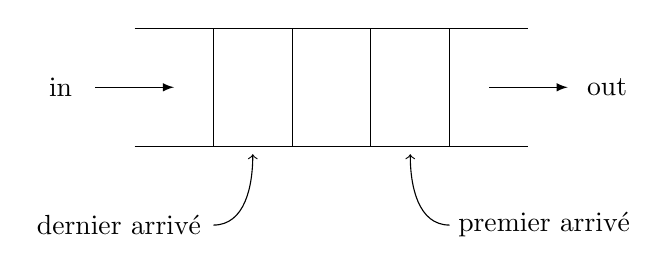
\begin{tikzpicture}
            \draw (0,0) -- (5,0);
            \draw (0,1.5) -- (5,1.5);
            \draw (1,0) -- (1,1.5);
            \draw (2,0) -- (2,1.5);
            \draw (3,0) -- (3,1.5);
            \draw (4,0) -- (4,1.5);
            \draw[-latex] (-0.5,0.75) -- (0.5,0.75);
            \draw[-latex] (4.5,0.75) -- (5.5,0.75);
            \node (tmp) at (-1, 0.75) {~in};
            \node (tmp) at (6, 0.75) {out};
            \draw[->] (1,-1) to[out=0, in=270] (1.5, -0.1);
            \draw[->] (4,-1) to[out=180, in=270] (3.5, -0.1);
            \node (tmp) at (-0.2, -1) {dernier arrivé};
            \node (tmp) at (5.2, -1) {premier arrivé};
        \end{tikzpicture}
    \end{center}

    \begin{block}{Interface}
        \begin{description}
            \item[ajouter] mettre un élément à la fin de la file
            \item[observer] obtenir le premier élément dans la file
            \item[extraire] retirer le premier élément de la file 
        \end{description}
    \end{block}
}

\frame{
    \frametitle{Parcours en largeur (Breadth-First Search)}

    Si on utilise une \enavant{file} pour implanter l'algorithme de parcours générique précédent on obtient un parcours particulier appelé \enavant{parcours en largeur} (aussi appelé en largeur d'abord).

    \exercice{%
        Effectuer un parcours en largeur du graphe suivant à partir de $v_0 = v_1$
        \begin{center}
            \begin{tikzpicture}
                \node (a) at (0,0) {$\sommet{}_3$};
                \node (b) at (3,0) {$\sommet{}_4$};
                \node (c) at (0,3) {$\sommet{}_1$};
                \node (d) at (3,3) {$\sommet{}_2$};

                \shiftdraw{d}{a}{-1pt}{1pt};
                \draw[-latex] (a) to[in=270, out=180, looseness=5] (a);

                \shiftdraw{c}{d}{0}{1.5pt};

                \shiftdraw{d}{b}{-1.5pt}{0};
            \end{tikzpicture}
        \end{center}
    }
}

\frame{
    \frametitle{Propriété fondamentale du parcours en largeur}

    \definition[plus court chemin]{%
        Soit $\graphedef{}$ un graphe, soient $\sommet{}$ et $\sommetb{}$ deux sommets de $\graphe{}$.
        Un chemin $\chemin{}$ de $\sommet{}$ à $\sommetb{}$ est un plus court chemin de $\sommet{}$ à $\sommetb{}$ si tout autre chemin $\chemin{}'$ de $\sommet{}$ à $\sommetb{}$ est tel que $\taille{\chemin{}'} \geq \taille{\chemin{}}$.
    }

    \definition[distance]{%
        On appelle distance de $\sommet{}$ à $\sommetb{}$ la longueur d'un plus court chemin de $\sommet{}$ à $\sommetb{}$.
        On la note $\distance{\sommet{}}{\sommetb{}}$.
    }

    \pause

    \proposition{%
        Durant un parcours en largeur, à tout instant, si $\sommet{}$ est marqué alors tous les sommets $\sommetb{}$ tels que $\distance{\sommet{}_0}{\sommetb{}} < \distance{\sommet{}_0}{\sommet{}}$ le sont déjà.
    }
}

\frame{
    \frametitle{Propriété fondamentale du parcours en largeur, suite}

    Conséquence de la proposition~: on découvre les sommets (on les marque) dans l'ordre de leur distance à $\sommet{}_0$.

    \begin{center}
        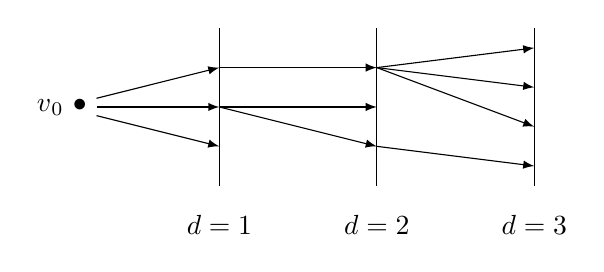
\begin{tikzpicture}
            \node (v0) at (-1,0) {$\sommet{}_0 ~\bullet$};
            \draw (1,1) -- (1,-1);
            \draw (3,1) -- (3,-1);
            \draw (5,1) -- (5,-1);
            \node (tmp) at (1,-1.5) {$d=1$};
            \node (tmp) at (3,-1.5) {$d=2$};
            \node (tmp) at (5,-1.5) {$d=3$};
            \draw[-latex] (v0) -- (1,0.5);
            \draw[-latex] (v0) -- (1,0);
            \draw[-latex] (v0) -- (1,-0.5);
            \draw[-latex] (1,0.5) -- (3,0.5);
            \draw[-latex] (1,0) -- (3,0);
            \draw[-latex] (1,0) -- (3,-0.5);
            \draw[-latex] (3,0.5) -- (5,0.75);
            \draw[-latex] (3,0.5) -- (5,0.25);
            \draw[-latex] (3,0.5) -- (5,-0.25);
            \draw[-latex] (3,-0.5) -- (5,-0.75);
        \end{tikzpicture}
    \end{center}

    \pause

    \exercice{%
        Prouver la proposition (on peut le faire par l'absurde).
    }
}

\frame{
    \frametitle{Parcours en largeur, autre version}

    \begin{center}
        \begin{minipage}{8.5cm}
            \begin{algorithmic}
                \In{$\graphedef{}$, $\sommet{}_0\in\sommets{}$}
                \only<2->{\Out{\enavant{pred}}}
                \State $t = init()$
                \State $t.ajouter(\sommet{}_0)$
                \State marquer $\sommet{}_0$
                \While{$!t.estVide()$}
                    \State $v = t.observer()$
                    \State $t.extraire()$
                    \ForAll{$\sommetb{}$ t.q $\exists (\sommet{}, \sommetb{})\in \arcs{}$, $\sommetb{}$ non marqué}
                        \State $t.ajouter(\sommetb{})$
                        \State marquer $\sommetb{}$
                        \only<2->{\State \enavant{$pred(\sommetb{}) = \sommet{}$}}
                    \EndFor
                \EndWhile
            \end{algorithmic}
        \end{minipage}
    \end{center}

    \only<2->{
        \proposition{%
            pred définit un routage par des plus courts chemins depuis $\sommet{}_0$ vers les sommets marqués.
        }
    }
}

\frame{
    \frametitle{Parcours en largeur, exercice et preuve}

    \exercice{%
        \begin{columns}
            \begin{column}{7cm}
                Soit le graphe suivant~:
                \begin{tikzpicture}
                    \node (v4) at (0,0) {$\sommet{}_4$};
                    \node (v5) at (3,0) {$\sommet{}_5$};
                    \node (v1) at (0,3) {$\sommet{}_1$};
                    \node (v2) at (3,3) {$\sommet{}_2$};
                    \node (v3) at (6,1.5) {$\sommet{}_3$};

                    \shiftdraw{v1}{v2}{0}{0};
                    \shiftdraw{v2}{v3}{0}{0};
                    \shiftdraw{v4}{v1}{0}{0};
                    \shiftdraw{v5}{v4}{0}{0};
                    \shiftdraw{v5}{v3}{0}{0};

                    \draw[-latex] (v2) to[in=45, out=135, looseness=5] (v2);
                \end{tikzpicture}
            \end{column}
            \begin{column}{4cm}
                \begin{itemize}
                    \item Faire pas à pas le parcours en largeur de ce graphe à partir de $\sommet{}_0 = \sommet{}_1$ et en calculant pred.
                    \item En déduire le plus court chemin de $\sommet{}_1$ à $\sommet{}_3$.
                \end{itemize}
            \end{column}
        \end{columns}
    }

    \pause

    \exercice{%
        Faire la preuve de la proposition précédente.
        On peut commencer par montrer que pred définit un routage et montrer ensuite que ce routage est par des plus courts chemins.
    }
}

\subsection{Parcours en profondeur}

\frame{
    \frametitle{Un tas particulier : la pile}

    Structure \enavant{LIFO} (Last In, First Out)

    \begin{columns}
        \begin{column}{5cm}
            \begin{center}
                \begin{tikzpicture}
                    \draw (0,0) -- (0,4.5);
                    \draw (2,0) -- (2,4.5);
                    \draw (0,0) -- (2,0);
                    \draw (0,1) -- (2,1);
                    \draw (0,2) -- (2,2);
                    \draw (0,3) -- (2,3);
                    \draw[-latex] (0.6,5) -- (0.6,4);
                    \draw[-latex] (1.4,4) -- (1.4,5);
                    \node (tmp) at (0.6, 5.25) {in};
                    \node (tmp) at (1.4, 5.25) {out};
                    \draw[->] (3,3.5) to[out=270, in=0] (2.1, 2.5);
                    \draw[->] (3,-0.5) to[out=90, in=0] (2.1, 0.5);
                    \node (tmp) at (3.5, 3.8) {dernier arrivé};
                    \node (tmp) at (3.5, -0.8) {premier arrivé};
                \end{tikzpicture}
            \end{center}
        \end{column}
        \begin{column}{6cm}
            \begin{block}{Interface}
                \begin{description}
                    \item[ajouter] mettre un élément au sommet de la pile
                    \item[observer] obtenir l'élément au sommet de la pile
                    \item[extraire] retirer l'élément au sommet de la pile
                \end{description}
            \end{block}
        \end{column}
    \end{columns}
}

\frame{
    \frametitle{Parcours en profondeur (Depth-First Search)}

    Si on utilise une \enavant{pile} pour implanter l'algorithme de parcours générique précédent on obtient un parcours particulier appelé \enavant{parcours en profondeur} (aussi appelé en profondeur d'abord).

    \exercice{%
        Effectuer un parcours en profondeur du graphe suivant à partir de $v_0 = v_1$
        \begin{center}
            \begin{tikzpicture}
                \node (a) at (0,0) {$\sommet{}_3$};
                \node (b) at (3,0) {$\sommet{}_4$};
                \node (c) at (0,3) {$\sommet{}_1$};
                \node (d) at (3,3) {$\sommet{}_2$};

                \shiftdraw{d}{a}{-1pt}{1pt};
                \draw[-latex] (a) to[in=270, out=180, looseness=5] (a);

                \shiftdraw{c}{d}{0}{1.5pt};

                \shiftdraw{d}{b}{-1.5pt}{0};
            \end{tikzpicture}
        \end{center}
    }
}

\frame{
    \frametitle{Propriétés du parcours en profondeur}

    \proposition{%
        À tout instant la pile (si elle n'est pas vide) définit un chemin de $\sommet{}_0$ au sommet $\sommet{}$ situé à son sommet.
    }

    \exercice{%
        Le prouver.
    }

    \pause

    \proposition{%
        Si $\sommet{}$ est dépilé, alors tous les sommets $\sommetb{}$ atteignables depuis $\sommet{}$ par un chemin $\sommet{}\cheminvers{}\sommetb{}$ ne passant par aucun sommet encore dans la pile sont marqués.
    }

    \exercice{%
        Le prouver.
    }
}

    \section{Chemins optimaux}

\frame{
    \frametitle{Définitons}

    \definition[graphe valué]{%
        Un graphe valué est un triplet $\grapheval{}$ où $(\sommets{}, \arcs{})$ est un graphe et $\cout{}: \arcs{}\rightarrow \mathbb{R}$ est une fonction de coût.
    }

    \definition[coût d'un chemin]{%
        Soit $\grapheval{}$ un graphe valué, soit $\chemin{} = \sommet{}_1,\dots,\sommet{}_n$ un chemin de $(\sommets{}, \arcs{})$, le coût de $\chemin{}$ est 
        $$\cout{}(\chemin{}) = \sum_{i=2}^{n}\cout{}((\sommet{}_{i-1}, \sommet{}_i))$$
    }

    \definition[chemin de coût minimal]{%
        Soit $\grapheval{}$ un graphe valué.
        Un chemin $\chemin{}$ de $\sommet{}$ à $\sommetb{}$ est un chemin de coût minimal si $\forall \chemin{}'$ chemin de $\sommet{}$ à $\sommetb{}$ on a $\cout{}(\chemin{}') \geq \cout{}(\chemin{})$.
    }
}

\frame{
    \frametitle{Les problèmes qu'on se pose}

    \definition[\pbvv{}]{%
        Trouver un chemin de coût minimal de $\sommet{}$ à $\sommetb{}$.
    }

    \definition[\pbvetoile{}]{%
        Pour tout $\sommetb{}$, trouver un chemin de coût minimal de $\sommet{}$ à $\sommetb{}$.
    }

    \definition[\pbetoileetoile{}]{%
        Pour tout $\sommet{}$ et tout $\sommetb{}$, trouver un chemin de coût minimal de $\sommet{}$ à $\sommetb{}$.
    }   
}

\frame{
    \frametitle{Les problèmes qu'on se pose, suite}

    \exercice{%
        \begin{center}
            \begin{tikzpicture}
                \node (v3) at (0,0) {$\sommet{}_3$};
                \node (v4) at (3,0) {$\sommet{}_4$};
                \node (v1) at (0,3) {$\sommet{}_1$};
                \node (v2) at (3,3) {$\sommet{}_2$};
                \node (v5) at (6,0) {$\sommet{}_5$};

                \shiftdraw{v1}{v2}{0}{0};
                \shiftdraw{v1}{v4}{0}{0};
                \shiftdraw{v2}{v4}{0}{0};
                \shiftdraw{v3}{v1}{0}{0};
                \shiftdraw{v4}{v3}{0}{0};
                \shiftdraw{v5}{v4}{0}{0}; 

                \node (info) at (1.5, 3.2) {2};
                \node (info) at (1.5, -0.2) {2};
                \node (info) at (-0.2, 1.5) {2};
                \node (info) at (3.2, 1.5) {2};
                \node (info) at (4.5, -0.2) {0};
                \node (info) at (1.7, 1.7) {-1};
            \end{tikzpicture}
        \end{center}

        \begin{itemize}
            \item Résoudre \pbvv{} pour $\sommet{}=\sommet{}_1$ et $\sommetb{}=\sommet{}_3$.
            \item Résoudre \pbvetoile{} pour $\sommet{}=\sommet{}_1$.
            \item Résoudre \pbetoileetoile{}.
        \end{itemize}
    }
}

\subsection{Depuis un sommet}

\frame{
    \frametitle{Circuits et chemins de coût minimal}

    \definition[circuit]{
        Soit $\graphedef{}$ un graphe. Un chemin de $\sommet{}$ à $\sommetb{}$ dans $\graphe{}$ est appelé circuit si $\sommet{} = \sommetb{}$.
    }

    \definition[circuit absorbant]{
        Un circuit $\chemin{}$ d'un graphe valué $\grapheval{}$ est dit absorbant si $\cout{}(\chemin{}) < 0$.
    }

    \pause

    \proposition{%
        Soit $\sommet{}$ un sommet d'un graphe (valué) $\graphe{}$.
        Le problème \pbvetoile{} admet une solution si et seulement si il n'existe pas de circuit absorbant atteignable depuis $\sommet{}$ dans $\graphe{}$.
    }
}

\frame{
    \frametitle{Preuve de la proposition}

    \proposition[lemme]{%
        Si un graphe $\graphe{}$ n'a pas de circuit absorbant alors pour tout chemin $\chemin{}$ de $\sommet{}$ à $\sommetb{}$ de $\graphe{}$ il existe un chemin $\chemin{}'$ extrait de $\chemin{}$ tel que~:
        \begin{itemize}
            \item $\chemin{}'$ est élémentaire,
            \item $\cout{}(\chemin{}') \leq \cout{}(\chemin{})$.
        \end{itemize}
    }

    \proposition[lemme]{%
        Dans tout graphe $\graphe{}$ il existe un nombre fini de chemins élémentaires.
    }

    \exercice[preuve de la proposition précédente]{%
        \begin{itemize}
            \item Prouver les deux lemmes.
            \item En déduire que si un graphe n'a pas de circuit absorbant alors \pbvetoile{} admet une solution.
            \item Montrer (par la contraposée) que si \pbvetoile{} admet une solution alors le graphe n'a pas de circuit absorbant.
        \end{itemize}
    }
}

\subsection{Algorithme de Bellman-Ford}

\frame{
    \frametitle{Présentation de l'algorithme de Bellman-Ford}

    L'algorithme de Bellamn-Ford calcule les chemins de coût minimal d'une source aux autres sommets dans un graphe valué, c'est-à-dire qu'il \enavant{résout \pbvetoile{}}.
    De plus, il \enavant{détecte les circuits absorbants}.
    
    \begin{center}
        \begin{minipage}{9cm}
            \begin{algorithmic}
                \In{$\grapheval{}$, $\sommet{}_0\in\sommets{}$}
                \Out{d, pred, vrai/faux}
                \State $d(\sommet{}_0) = 0, \forall \sommet{}\in\sommets{}, \sommet{}\neq\sommet{}_0, d(\sommet{}) = +\infty$
                \For{$\taille{\sommets{}} - 1$ fois}
                    \ForAll{$(\sommet{}, \sommetb{})\in \arcs{}$}
                        \If{$d(\sommetb{}) > d(\sommet{}) + \cout{}((\sommet{}, \sommetb{}))$}
                            \State $d(\sommetb{}) = d(\sommet{}) + \cout{}((\sommet{}, \sommetb{}))$ \enavant{// relachement}
                            \State $pred(\sommetb{}) = \sommet{}$
                        \EndIf
                    \EndFor
                \EndFor
                \ForAll{$(\sommet{}, \sommetb{})\in \arcs{}$}
                    \If{$d(\sommetb{}) > d(\sommet{}) + \cout{}((\sommet{}, \sommetb{}))$}
                        \State {\bf return} faux
                    \EndIf
                \EndFor
                \State {\bf return} vrai
            \end{algorithmic}
        \end{minipage}
    \end{center}
}

\frame{
    \frametitle{Exemple}

    \exercice{%
        Appliquer l'alogrithme de Bellman-Ford au graphe suivant pour $\sommet{}_0 = \sommet{}_1$.
        \begin{center}
            \begin{tikzpicture}
                \node (v3) at (0,0) {$\sommet{}_3$};
                \node (v4) at (3,0) {$\sommet{}_4$};
                \node (v1) at (0,3) {$\sommet{}_1$};
                \node (v2) at (3,3) {$\sommet{}_2$};
                \node (v5) at (6,0) {$\sommet{}_5$};

                \shiftdraw{v1}{v2}{0}{0};
                \shiftdraw{v1}{v4}{0}{0};
                \shiftdraw{v2}{v4}{0}{0};
                \shiftdraw{v3}{v1}{0}{0};
                \shiftdraw{v4}{v3}{0}{0};
                \shiftdraw{v5}{v4}{0}{0}; 

                \node (info) at (1.5, 3.2) {2};
                \node (info) at (1.5, -0.2) {2};
                \node (info) at (-0.2, 1.5) {2};
                \node (info) at (3.2, 1.5) {2};
                \node (info) at (4.5, -0.2) {0};
                \node (info) at (1.7, 1.7) {-1};
            \end{tikzpicture}
        \end{center}
    }
}

\frame{
    \frametitle{Coût d'un chemin de coût minimal}

    \notation{%
        Dans un graphe $\graphe{}$, pour tout $\sommet{}$ et tout $\sommetb{}$, on note $\coutmin{\sommet{}}{\sommetb{}}$ le coût d'un chemin de coût minimal de $\sommet{}$ à $\sommetb{}$.
    }

    \remarque{%
        Ce coût peut être $+\infty$ s'il n'existe pas de chemin de $\sommet{}$ à $\sommetb{}$.
        Il peut être $-\infty$ s'il y a un circuit absorbant sur un chemin de $\sommet{}$ à $\sommetb{}$ (dans ce cas on fait un léger abus car le coût infini n'est atteint que par un chemin infini, qui n'existe pas d'après notre définition des chemins).
    }
}

\frame{
    \frametitle{Preuve de l'algoritme de Bellman-Ford}

    Notre objectif dans cette partie est de prouver l'algorithme de Bellman-Ford, c'est-à-dire de prouver la proposition suivante.

    \proposition[validité de l'algoritme de Bellman-Ford]{%
        Soit $\grapheval{}$ un graphe valué et soit $\sommet{}_0$ un sommet de $\graphe{}$.
        \begin{itemize}
            \item Si $\graphe{}$ ne contient pas de circuit absorbant atteignable depuis $\sommet{}_0$, alors l'algorithme de Bellman-Ford retourne \enavant{vrai} et on a $d(\sommet{}) = \coutmin{\sommet{} 0}{\sommet{}}$ pour tout $\sommet{}$.
            \item Si $\graphe{}$ contient un circuit absorbant atteignable depuis $\sommet{}_0$, alors l'algorithme de Bellman-Ford retourne \enavant{faux}.
        \end{itemize}
    }

    Pour pouvoir prouver cette proposition on va d'abord prouver un certain nombre de lemmes.
}

\frame{
    \frametitle{Borne supérieure}

    \proposition[borne supérieure]{%
        À tout moment durant l'exécution de l'algorithme on a $d(\sommet{}) \geq \coutmin{\sommet{}_0}{\sommet{}}$ et, si on arrive à $d(\sommet{}) = \coutmin{\sommet{}_0}{\sommet{}}$, alors $d(\sommet{})$ ne changera plus jamais.
    }

    \exercice{%
        Prouver cette proposition.
        On peut faire la preuve par induction sur le nombre de relachements.
    }
}

\frame{
    \frametitle{Relachement des chemins}

    \proposition[relachement des chemins]{%
        Supposons que $\graphe{}$ n'a pas de circuits absorbants.
        Soit $\chemin{}=\sommet{}_0\sommet{}_1\dots\sommet{}_n$ un chemin de coût minimal de $\sommet{}_0$ à $\sommet{}_n$.
        N'importe quelle séquence de relachements qui inclue, dans cet ordre, les relachements de $(\sommet{}_0, \sommet{}_1)$, $(\sommet{}_1, \sommet{}_2)$, \dots et $(\sommet{}_{n-1}, \sommet{}_n)$ produit $d(\sommet{}_n) = \coutmin{\sommet{}_0}{\sommet{}_n}$ après ces relachements (et pour toujours après cela).
    }

    \exercice{%
        Prouver cette proposition.
        On pourra le faire par induction sur les sommets de $\chemin{}$.
    }
}

\frame{
    \frametitle{Correction}

    \proposition[correction]{%
        Soit $\graphe{}$ un graphe valué et $\sommet{}_0$ un sommet de $\graphe{}$ tel qu'il n'y a pas de circuits absorbants atteignables depuis $\sommet{}_0$.
        Après avoir exécuté l'algorithme de Bellman-Ford on a $d(\sommet{}) = \coutmin{\sommet{}_0}{\sommet{}}$ pour tout $\sommet{}$ atteignable depuis $\sommet{}_0$.
    }

    \exercice{%
        Prouver cette proposition.
        On pourra notamment utiliser pour cela la proposition \emph{relachement des chemins}.
    }

    \pause

    \proposition[corollaire]{%
        Un sommet $\sommet{}$ termine avec $d(\sommet{}) = +\infty$ si et seulement si $\sommet{}$ n'est pas atteignable depuis $\sommet{}_0$. 
        (Ceci est valable même en présence de circuits absorbants.)
    }

    \exercice{%
        Prouver ce corollaire.
    }
}

\frame{
    \frametitle{Preuve de l'algorithme de Bellman-Ford, enfin}

    \exercice{%
        À partir des propositions précédentes prouver la validité de l'algorithme de Bellman-Ford.
        \begin{itemize}
            \item Pour le cas sans circuits absorbants il suffit d'utiliser la \emph{correction} et de prouver qu'on retourne vrai dans ce cas.
            \item Pour le cas avec circuits absorbants on peut procéder par contradiction (en supposant que l'algorithme retourne vrai et en étudiant la deuxième boucle pour aboutir à la contradiction).
        \end{itemize}
    }
}

\frame{
    \frametitle{Complexité}

    \exercice{%
        \begin{enumerate}
            \item Quelle est la complexité de l'algorithme de Bellman-Ford ?
            \item Justifier que l'on peut arrêter l'algorithme dès qu'aucun relachement n'a d'effet lors d'un tour de boucle.
            \item Quelle est alors la complexité de l'algorithme ?
        \end{enumerate}
    }

}

\subsection{Algorithme de Dijkstra}

\end{document}